\documentclass[border=3mm]{standalone}

\usepackage{xcolor}

\definecolor{palesilver}{rgb}{0.79, 0.75, 0.73}
\definecolor{silver}{rgb}{0.75, 0.75, 0.75}
\definecolor{goldenbrown}{rgb}{0.6, 0.4, 0.08}
\definecolor{glaucous}{rgb}{0.38, 0.51, 0.71}
\usepackage{tikz}
\usetikzlibrary{shapes,decorations,shadows}

\usetikzlibrary{calc}


\usetikzlibrary{decorations.text}



\begin{document}


\tikzset{paint/.style={ draw=#1!50!black, fill=#1!50 },
    decorate with/.style=
    {decorate,decoration={shape backgrounds,shape=#1,shape size=2mm}}}




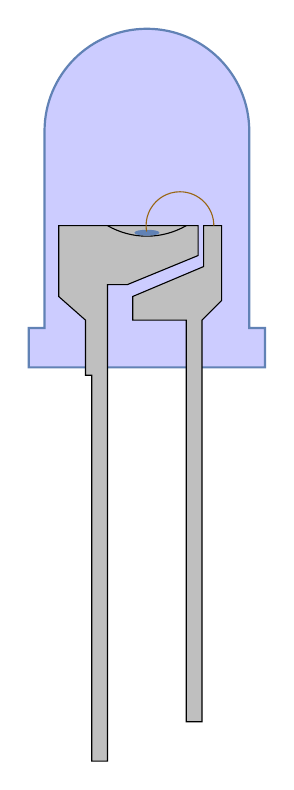
\begin{tikzpicture}
 %\draw[help lines] (0,-1) grid (3,6); 
 % LED Plastik Gehäuse
 \draw[thick,color=glaucous,fill=blue!20] (0,1) -- (3,1) -- (3,1.5) -- (2.8,1.5) -- (2.8,4) arc (0:180:1.3) -- (0.2,1.5) -- (0,1.5) -- cycle;
 % Anode
 \draw[thin,color=black,fill=silver] (2,-3.5) -- (2.2,-3.5) --(2.2,1.6) -- (2.45,1.85) -- (2.45,2.8) -- (2.22,2.8) -- (2.22,2.28) -- (1.32,1.9) -- (1.32,1.6) -- (2,1.6) --cycle;
 % Kathode
 \draw[thin,color=black,fill=silver] (1,-4) -- (1,2.05) -- (1.25,2.05) -- (2.15,2.42) -- (2.15,2.8) --  (0.38,2.8) -- (0.38,1.9) -- (0.72,1.6) -- (0.72,0.9) -- (0.8,0.9) -- (0.8,-4) -- cycle ; 
 % Reflektor
 \draw (2,2.8) arc (-60:-120:1) ;
 % Kristall
 \draw[color=glaucous,fill=glaucous] (1.5,2.71) ellipse [x radius = .15, y radius = .03,
  start angle = 30, end angle = 150];
 % Draht
 \draw[color=goldenbrown] (2.35,2.8) arc (0:190:0.43); 
\end{tikzpicture}


\end{document}